\documentclass[10pt,a4paper,twocolumn,landscape]{article}

\usepackage{polyglossia}
\setmainlanguage{russian}
\setotherlanguage{english}
\usepackage{amsmath,amssymb,mathspec}
\usepackage{soul}
\usepackage{pgf,tikz,pgfplots}
\usepackage{wrapfig,graphicx}
\usepackage{fancyhdr,lastpage,array}
\usepackage{multirow,multicol,enumitem}
\usepackage[top=2.5cm, bottom=2cm, left=2.2cm, right=1.5cm]{geometry}
\usepackage{pgffor}
\usepackage{makecell}
\usepackage{graphicx}
\usepackage{enumitem}
\graphicspath{ {./bio/images/} }

% Set fonts
%\setmainfont{Times New Roman}
\setmainfont[Scale=1]{PT Serif}
%\setmathrm[Scale=0.8]{Cascadia Code PL} % for \sin, \cos, ...
\usepackage[euler-digits,euler-hat-accent]{eulervm}
\usepackage[mathscr]{euscript}
\setallsansfonts{PT Sans}
\setallmonofonts[Scale=0.95]{PT Mono}

\setlist[enumerate]{nosep}

\everymath{\displaystyle}
\newcommand{\Z}{\mathcal{Z}}
\newcommand{\Q}{\mathcal{Q}}
\newcommand{\N}{\mathcal{N}}
\newcommand{\No}{\mathcal{N}_0}
\newcommand{\R}{\mathcal{R}}

\pgfplotsset{compat=newest}

\setlength{\parindent}{0cm}

\setlength{\columnsep}{2.5cm}
\setlength{\columnwidth}{11.3cm}

\renewcommand{\headrulewidth}{0cm}
\renewcommand{\footrulewidth}{0cm}
\renewcommand{\headruleskip}{0.6cm}
\renewcommand{\footruleskip}{0cm}
\renewcommand{\theenumii}{\Asbuk{enumi}}

\newcommand{\PreserveBackslash}[1]{\let\temp=\\#1\let\\=\temp}
\newcolumntype{C}[1]{>{\PreserveBackslash\centering}p{#1}}
\newcolumntype{R}[1]{>{\PreserveBackslash\raggedleft}p{#1}}
\newcolumntype{L}[1]{>{\PreserveBackslash\raggedright}p{#1}}


% \createpart{2} -> Часть 2
\newcommand{\createpart}[1]{ \center{\textsf{\textbf{Часть #1}}} }

% \createtask{2}{text} -> [2] text
\newcommand{\createtask}[2]{
	\hspace{-1.3cm}
	\begin{tabular}{c l}
		\framebox[0.85cm]{\textsf{\textbf{#1}}}\hspace{-0.15cm} &
		\begin{minipage}[t]{11.25cm}
			#2
		\end{minipage}
	\end{tabular}
	\phantom{1}
}

% \blankanswer -> [4.5cm] line
\newcommand{\blankanswer}{ \underline{\hspace{4.5cm}} }

% \partbox{text} -> [text]
\newcommand{\partbox}[1]{
	\hspace{-0.3cm}
	\framebox[11.5cm]{
		\begin{minipage}[l]{11.2cm}
			\vspace{-1em}\phantom{1}\\
			\textsf{\textit{\textbf{ #1 }}}
			\vspace{-0.1cm}
		\end{minipage}
	}
	\phantom{1}
}

\newcommand{\taskbox}[1]{
	\hspace{-0.3cm}
	\framebox[11.5cm]{
		\begin{minipage}[l]{11.2cm}
			\vspace{-1em}\phantom{1}\\
			\textsf{ #1 }
			\vspace{-0.1cm}
		\end{minipage}
	}
	\phantom{1}
}	

% \createheaders -> set up fancyhdr
\makeatletter
\newcommand{\createheaders}{
	\raggedbottom
	\pagestyle{fancy}
	\fancypagestyle{plain}{}
	\setlength{\headheight}{0cm}
	\fancyhead[L]{
		\scriptsize
		\textsf{ 
			\begin{tabular}{L{4.2cm} R{4.2cm} R{1.9cm}}
				\hspace{-0.1cm}\@title & \@author & \thepage/\pageref{LastPage}
			\end{tabular}
		}
	}
	\fancyhead[R]{\textsf{\scriptsize \@title\hspace{0.4cm}}}
	\fancyfoot[L]{
		\hspace{0.5cm}
		\begin{minipage}[l]{11.5cm}
			\center{
				\textsf{
					\tiny
					Создано командой 4GIA - с любовью.
					\\[-0.2cm]
					Копирование \textbf{допускается}
				}
			}
		\end{minipage}
	}
	\fancyfoot[C]{}
}
\makeatother

% \separ -> 1cm
\newcommand{\separ}{\vspace{1em}}

% \sepline -> 1em
\newcommand{\sepline}{\vspace{1em}}



\title{Открытый вариант}
\author{БИОЛОГИЯ}


\begin{document}

\begin{center}
	\textsf{\textbf{Единый государственный экзамен по БИОЛОГИИ \\
	Инструкция по выполнению работы \\}}
	\sepline
	Экзаменационная работа состоит из двух частей, включающих в себя
	29 заданий. Часть 1 содержит 22 задания с кратким ответом. Часть 2
	содержит 7 заданий с развёрнутым ответом. \\
	На выполнение экзаменационной работы по биологии отводится 3 часа
	55 минут (235 минут). \\
	Ответами к заданиям части 1 (1–22) являются последовательность
	цифр, число или слово (словосочетание). Ответы запишите по приведённым
	ниже \underline{образцам} в поле ответа в тексте работы без пробелов, запятых и других
	дополнительных символов, а затем перенесите в бланк ответов № 1.


\taskbox{
\text{Ответ в КИМ:}
\begin{tabular}{|c|c|}
	\hline
	3 & 5 \\
	\hline
\end{tabular} \text{Ответ в бланке:} \begin{tabular}{|c|c|c|c|c|}
	\hline
	3 & 5 & & &\\
	\hline
\end{tabular} \\ 
\text{Ответ в КИМ:}
	\begin{tabular}{|c|c|}
		\hline
		X & Y \\
		\hline
		3 & 5 \\
		\hline
	\end{tabular} \text{Ответ в бланке:} \begin{tabular}{|c|c|c|c|c|}
		\hline
		3 & 5 & & &\\
		\hline
		\end{tabular} \\
\text{Ответ в КИМ:} \underline{   3,5    }
\text{Ответ в бланке:} \begin{tabular}{|c|c|c|c|c|}
			\hline
			3 & , & 5 & &\\
			\hline
			\end{tabular} \\
\text{Ответ в КИМ:} \underline{ЖЕЛЕЗА}
\text{Ответ в бланке:} \begin{tabular}{|c|c|c|c|c|c|}
			\hline
			Ж & Е & Л & Е & З & А \\
			\hline
			\end{tabular} \\
}
\sepline \\
Ответы к заданиям 29–34 включают в себя подробное описание всего хода выполнения задания. В бланке ответов № 2 укажите номер задания
и запишите его полное решение. \\
Все бланки ЕГЭ заполняются яркими чёрными чернилами.
Допускается использование гелевой или капиллярной ручки. \\
При выполнении заданий можно пользоваться черновиком. \textbf{Записи
в черновике, а также в тексте контрольных измерительных материалов
не учитываются при оценивании работы.} \\ 
При выполнении работы используйте Периодическую систему химических элементов Д.И. Менделеева, таблицу растворимости солей, кислот и оснований в воде, электрохимический ряд напряжений металлов. Эти сопроводительные материалы прилагаются к тексту работы.\\ 
Для вычислений используйте непрограммируемый калькулятор. \\
Баллы, полученные Вами за выполненные задания, суммируются. Постарайтесь выполнить как можно больше заданий и набрать наибольшее количество баллов. \\
После завершения работы проверьте, чтобы ответ на каждое задание в бланках ответов № 1 и № 2 был записан под правильным номером. \\
\textit{\textsf{\textbf{Желаем успеха!}}}
\end{center}
			
\createheaders

\createpart{1}
\partbox{
	Ответами к заданиям 1--22 являются последовательность цифр или букв.
	Ответ запишите в поле ответа в тексте работы, а затем
	перенесите в БЛАНК ОТВЕТОВ № 1 справа от номера
	соответствующего задания, начиная с первой клеточки. Каждый символ
	пишите в отдельной клеточке в соответствии с приведёнными в бланке
	образцами.
}
\separ


\foreach \num in {1, 2, 3, 4}{
\createtask{\num}{\input{bio/task-\num}}\\
\separ}
\partbox{
	Рассмотрите рисунок и выполните задания 5 и 6. \\
		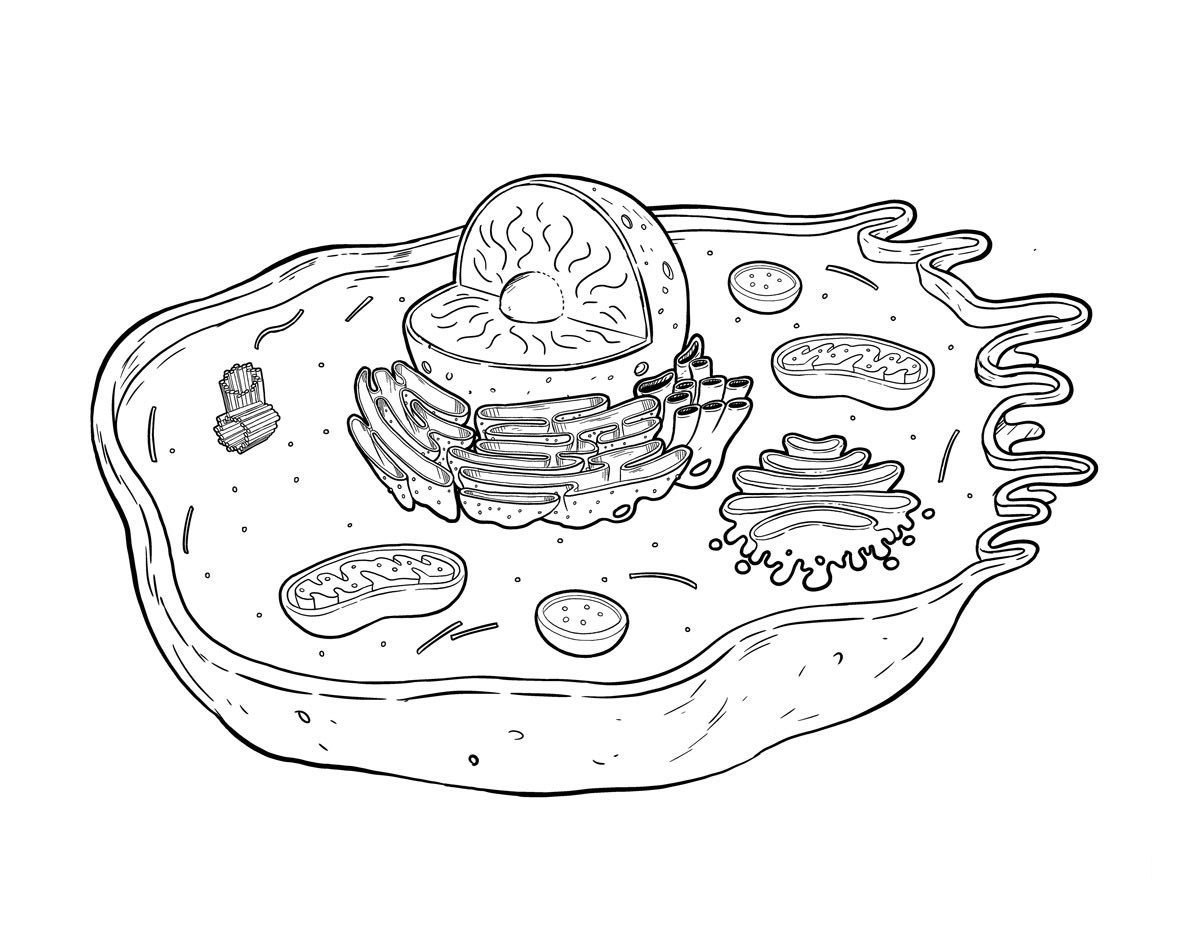
\includegraphics[height=6cm, width=8cm]{bio/images/cell.jpg}
} \\ \separ 
\foreach \num in {5, 6, ..., 12}{
\createtask{\num}{\input{bio/task-\num}}\\
\separ}
\partbox{
	Рассмотрите рисунок и выполните задания 13 и 14. \\
		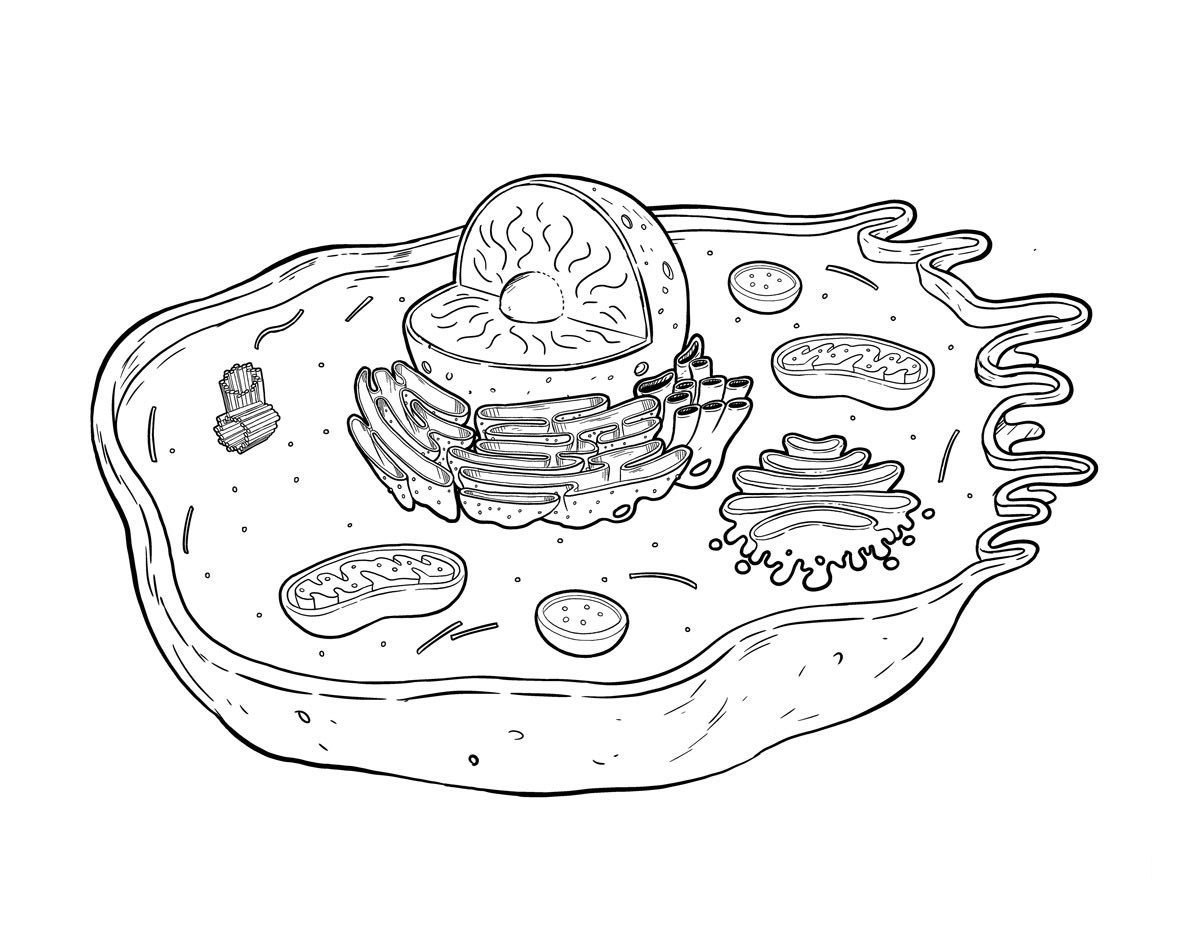
\includegraphics[height=6cm, width=8cm]{bio/images/cell.jpg}
} \\ \separ

\foreach \num in {13, 14, ..., 22}{
\createtask{\num}{\input{bio/task-\num}}\\
\separ}

\separ

\partbox{
	В бланк ответов № 1 перенесите только числа, не разделяя их пробелом
	или другим знаком.
} 

\pagebreak

\createpart{2}
\\
\partbox{
	Для записи ответов на задания 22--29 используйте БЛАНК
	ОТВЕТОВ № 2. Запишите сначала номер задания (24, 25 и т.д.), а затем
	решение соответствующей задачи. Ответы записывайте чётко
	и разборчиво.	
} \\
\separ
\partbox{
	Прочитайте описание эксперимента и выполните задания 23 и 24.
}
\\
\separ
Здесь должен был быть текст описания эксперимента, но так как это тестовый вариант - его здесь не будет. Зато будет очень длинный текст для того чтобы проверить, как он будет разбит и не слетит ли от этого форматирование. Я обожаю \LaTeX и очень хорошо пишу ужасный, просто отвратительный код. Как я это делаю? Откажусь от комментариев.\\
\separ 
\foreach \num in {23, 24, ..., 29}{
\createtask{\num}{\input{bio/task-\num}}\\
\separ}


\end{document}
